
{\underline {\bf В четвертой главе}} описано программное обеспечение, которое
было использовано для проведения тестировании, приведены результаты
тестирования, на основании которых проведено практическое сравнение АКМ
и разработанной модели.

Тесты проводились на новейшем множестве данных MovieLens Small.
Эти исходные данные были собраны компанией MovieLens, которая
занимается исследованиями и разработками в области РС. Исходные
данные являются данными,
которые были заполнены реальными
пользователями. Характеристики используемого множества данных:
\begin{itemize}
	\item $|U| = 700$;
	\item $|I| = 9000$ --- объектами являются фильмы
	\item $|P| = 100 000$ --- значениями $\rho(u, i)$ являются оценки
		пользователей, которые были ими заданы в соответствии со своим
		предпочтением к конкретному фильму;
	\item $|Y|$ --- характеристиками объектов являются кинематографические
		жанры;
	\item $X = I$ --- характеристиками пользователей для АКМ являются объекты.
\end{itemize}

Для АКМ $X = I$ и $w_U(u, x) = \rho(u,x), x \in I$.

Для задания правила вывода $\Pi_f$ была аналитически определена
функция $\delta_c$, основываясь на эвристическом предположении о том,
что между оценкой близости $\rho(u, i)$, заданной пользователем $u$
и характеристикой $y \in Y$ объекта $i$,
то есть жанром фильма, существует корреляция:
\begin{multline}
	\delta_c(i, y) = \frac{1}{|\{i: \exists \rho(u,i)\}|}
	\cdot
	|\{ i : (\rho(u, i) < \varepsilon_1) \wedge (\nu(y) = 1)\}| -\\
	|\{ i : (\rho(u, i) > \varepsilon_2) \wedge (\nu(y) = 1)\}|, \\
	\text{ где }
	\varepsilon_1 = 0,2, \varepsilon_2 = 0,6;
\end{multline}

Такое эвристическое предположение верно не для всех пользователей, так как
их вкусы могут быть неоднородными. Поэтому для некоторых пользователей функция
$\delta_c$ задана так, что
$|\rh(u, i_{\bot}) - \rho(u, i_{\bot}) \le \varepsilon_p|$,
а для некоторых --- нет.

Для проведения тестов исходные данные были
стандартно разбиты на тестовое и обучающее множество по следующему принципу:
разбиение проводилось случайно, в обучающее множество входит
80\% данных, в тестовое --- оставшиеся 20\%.

{\bf Сравнение моделей по критерию вычислительной сложности} \\
В качестве показателя вычислительной сложности алгоритма рассмотрим время,
которое затрачивается в среднем на решение задачи для одного пользователя.
Решение задачи $topN$ рассмотрим для $N = 10$, решение задачи $pred$
для одного прогнозируемого объекта. Алгоритмы использовались те же, что
применялись при определении качества решения, описанные выше.
Для оценки качества решения задачи $topN$ использовалась функция $1 -
\text{точность}$, для решения задачи $pred$ --- $NMAE$.

Тесты проводились на следующем оборудовании:
\begin{itemize}
	\item ОС --- Ubuntu 16.04 LS, 64 бита;
	\item Оперативная память --- 8Gb;
	\item Процессор --- Intel Core i5-4460 CPU @ 3.20GHz $\times$ 4;
\end{itemize}

\begin{table}[htb]
	\caption{Время решения задачи $topN$}
  \begin{center}
	\label{table:time-topn}
	\begin{tabular}{|c|c|}
	  \hline
		Модель & Время (с)\\ \hline
		ООМ& 13\\ \hline
		НРС&0,06 \\ \hline
	\end{tabular}
  \end{center}
\end{table}
%Столь длительное по времени решение задачи $topN$
%объясняется тем, что для решения этой задачи ведется работа
%с матрицей $\mathcal{M}$, в которой хранятся значения
%$\di$, по алгоритму приходится делать $|I|$ запросов к базе, по которому
%достается $|I|$ значений. Хранить целиком в памяти матрицу не оптимально по
%отношению к расходуемой оперативной памяти, а для реальных систем и вовсе может
%быть невозможно, где мощность множества объектов велика. Конечно,
%каждый шаг алгоритма можно оптимизировать и задействовать методы, ускоряющие
%работу алгоритма, однако целью исследования было сравнить стандартные
%предлагаемые подходы, а не оптимизировать по времени существующие.

\begin{table}[htb]
\caption{Время решения задачи $pred$}
  \begin{center}
	\label{table:time-p}
	\begin{tabular}{|c|c|}
	  \hline
		Модель & Время (с)\\ \hline
		СОМ& 0,5\\ \hline
		НРС&0,08 \\ \hline
	\end{tabular}
  \end{center}
\end{table}

В НРС определены алгоритмы, которые заметно эффективней
по критерию вычислительной сложности.
Практические результаты подтверждают вывод о том, что НРС является
эффективным расширением АКМ по критерию вычислительной сложности.

{\bf Влияние свойства транзитивности на ООМ при решении задачи $topN$} \\
Задача $topN$ решалась в ООМ при применении меры сходства единица минус косинус в качестве
$\rhi$ и $\varepsilon_i \in \{0,49; 0,1\}$.
При $\varepsilon_i = 0,1$ вероятность того, что $(i \rt j) \wedge (j \rt k)
\Rightarrow (i \rt k)$, выше, чем при $\varepsilon_i = 0,49$.
На Рис. \ref{pic:topn_trans} приведены результаты решений задачи $topN$ при
различных пороговых значениях. Черным цветом приведены результаты для
$\varepsilon_i = 0,1$, красным --- для $\varepsilon_i = 0,49$.
Видно, что при $\varepsilon_i = 0,1$ результаты решений эффективней.

Некоторые результаты при $\varepsilon_i = 0,1$ хуже, чем при
$\varepsilon_i = 0,49$. Это происходит для тех пользователей,
для которых характерно свойство неоднородности.

\begin{figure}[H]
	\caption{Влияние свойства транзитивности на ООМ при решении задачи $topN$}
	\label{pic:topn_trans}
	\begin{center}
		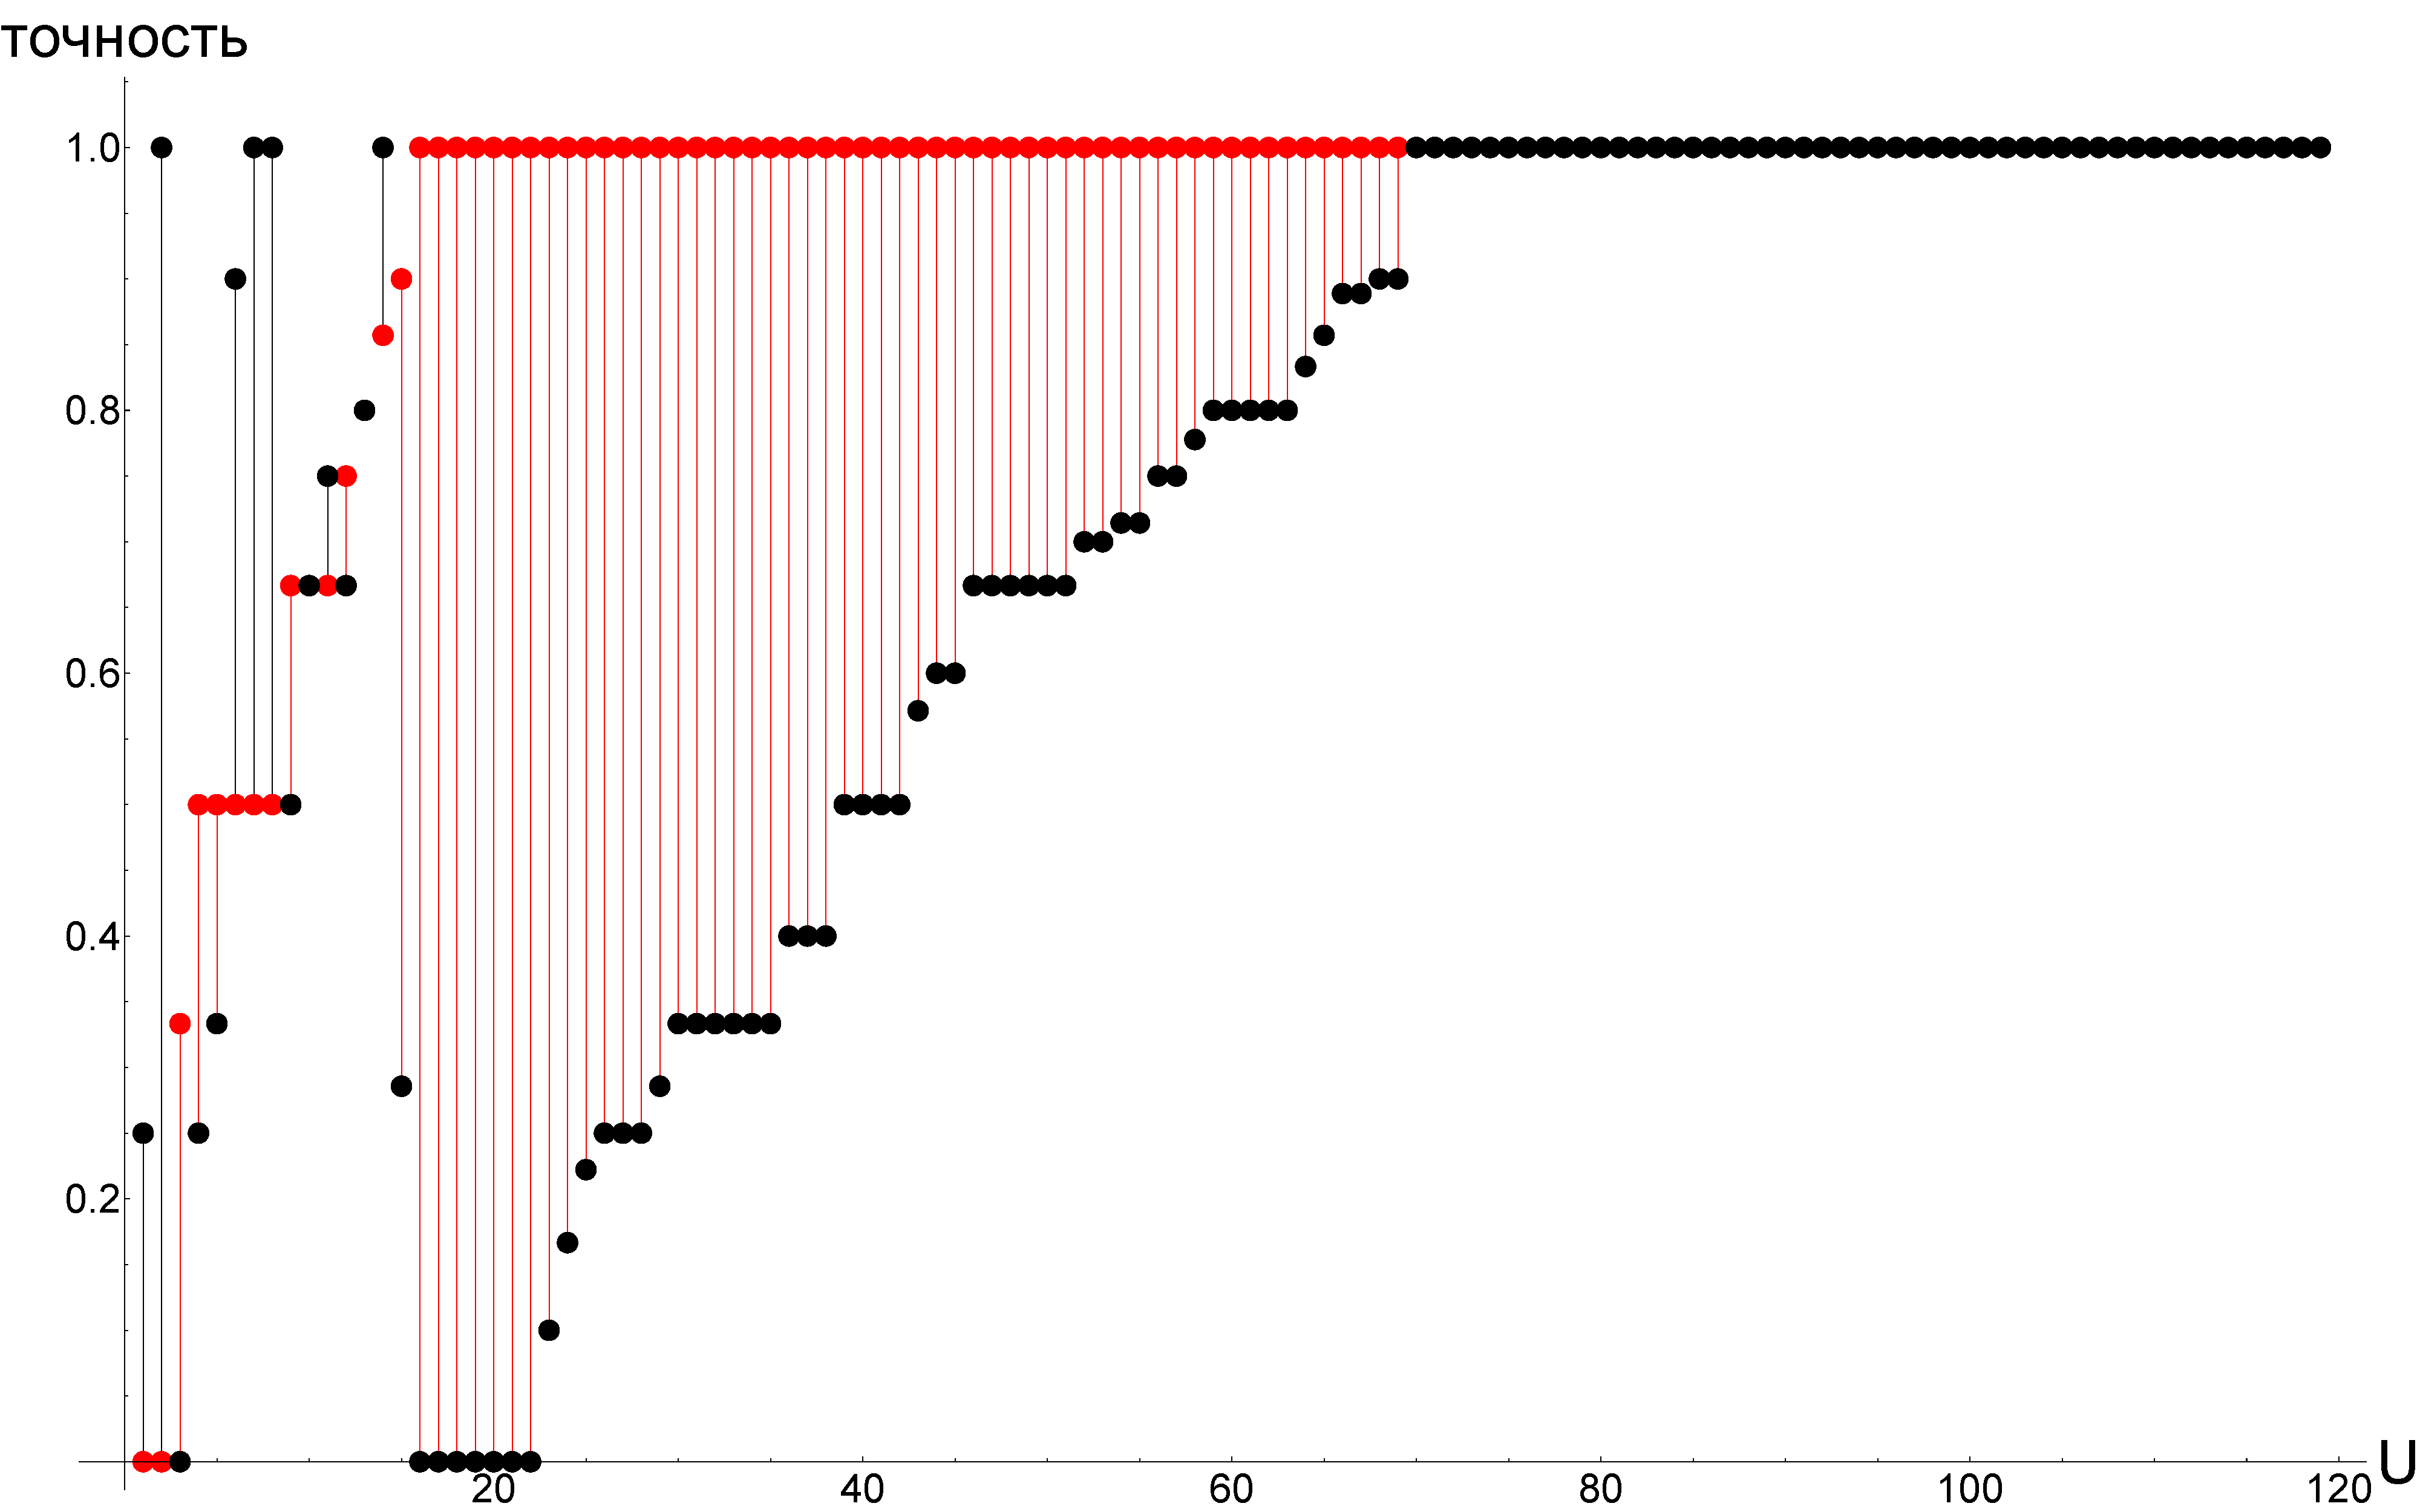
\includegraphics[width=5in,height=2in]{pics/results/transitivity.pdf}
\end{center}
\end{figure}

{\bf Влияние свойства транзитивности на СОМ при решении задачи $pred$} \\
Задача $pred$ была решена в РОМ при применении меры сходства
единица минус коэффициент корреляции Пирсона в качестве $\rhu$ и
$\varepsilon_p = \{0,49; 0,1\}$.
При $\varepsilon_p = 0,1$ вероятность того, что $(i \ru j) \wedge (j \ru k)
\Rightarrow (i \ru k)$, выше, чем при $\varepsilon_p = 0,49$.
На Рис. \ref{pic:pred_trans} приведены результаты решений задачи $pred$ при
различных пороговых значениях. Черным цветом приведены результаты для
$\varepsilon_p = 0,1$, красным --- для $\varepsilon_p = 0,49$.
Видно, что при $\varepsilon_p = 0,1$ результаты решений эффективней.

\begin{figure}[H]
	\caption{Влияние свойства транзитивности на СОМ при решении задачи $pred$}
	\label{pic:pred_trans}
	\begin{center}
		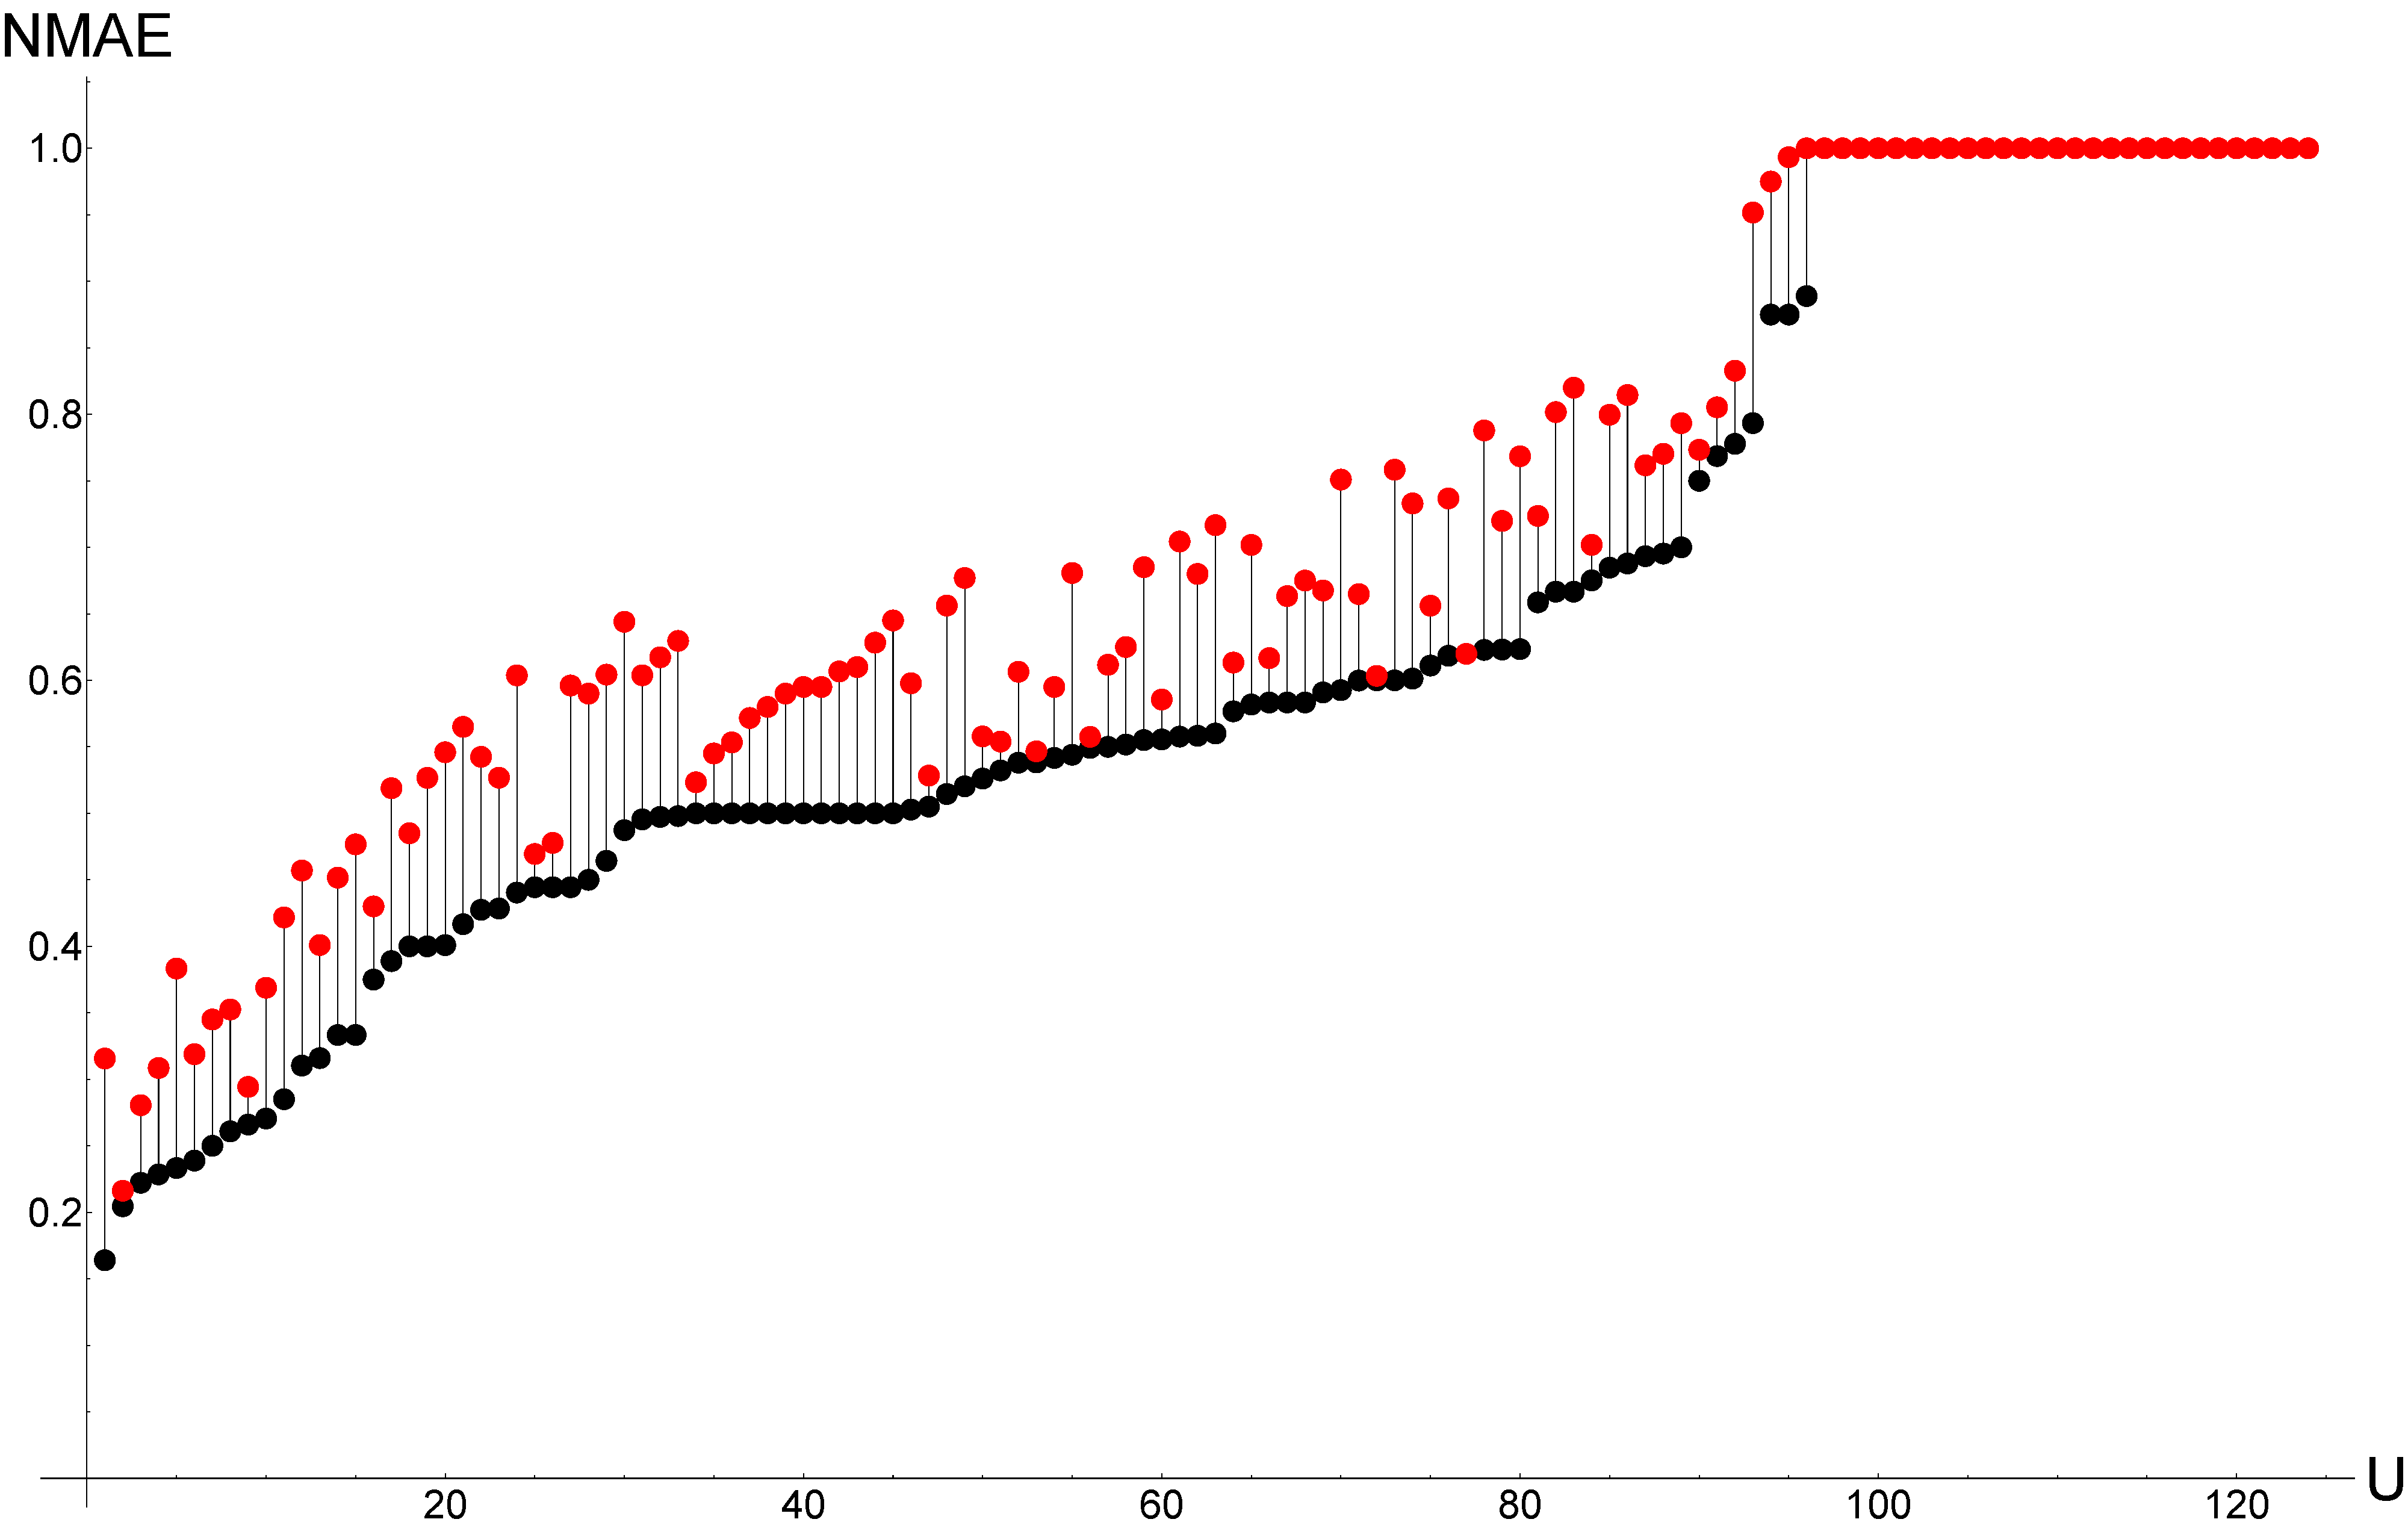
\includegraphics[width=5in,height=2in]{pics/results/ub_transitivity.pdf}
\end{center}
\end{figure}

%TODO: для задачи топн объяснить так, почему иногда хуже при применении
% п_о: в силу свойства неоднородности. На самом деле это говорит о том,
% что модель работает хорошо

%TODO: Написать, что оценки качества коррелируют меж собой, поэтому используем
%один показатель
{\bf Качество решений задачи $topN$ к при использовании $\Pi_O$ в НРС и ООМ}\\
На Рис. \ref{pic:topn_pio} приведены результаты решения
задачи $topN$ при применении $\Pi_O$ в ООМ и НРС.
Черным цветом обозначены результаты решения в НРС.
Видно, что в большинстве НРС более эффективна по критерию качества,
в других ситуациях предпочтения пользователя неоднородны.

\begin{figure}[H]
	\caption{Качество решений задачи $topN$ при использовании $\Pi_O$ в ООМ и
	НРС}
	\label{pic:topn_pio}
	\begin{center}
		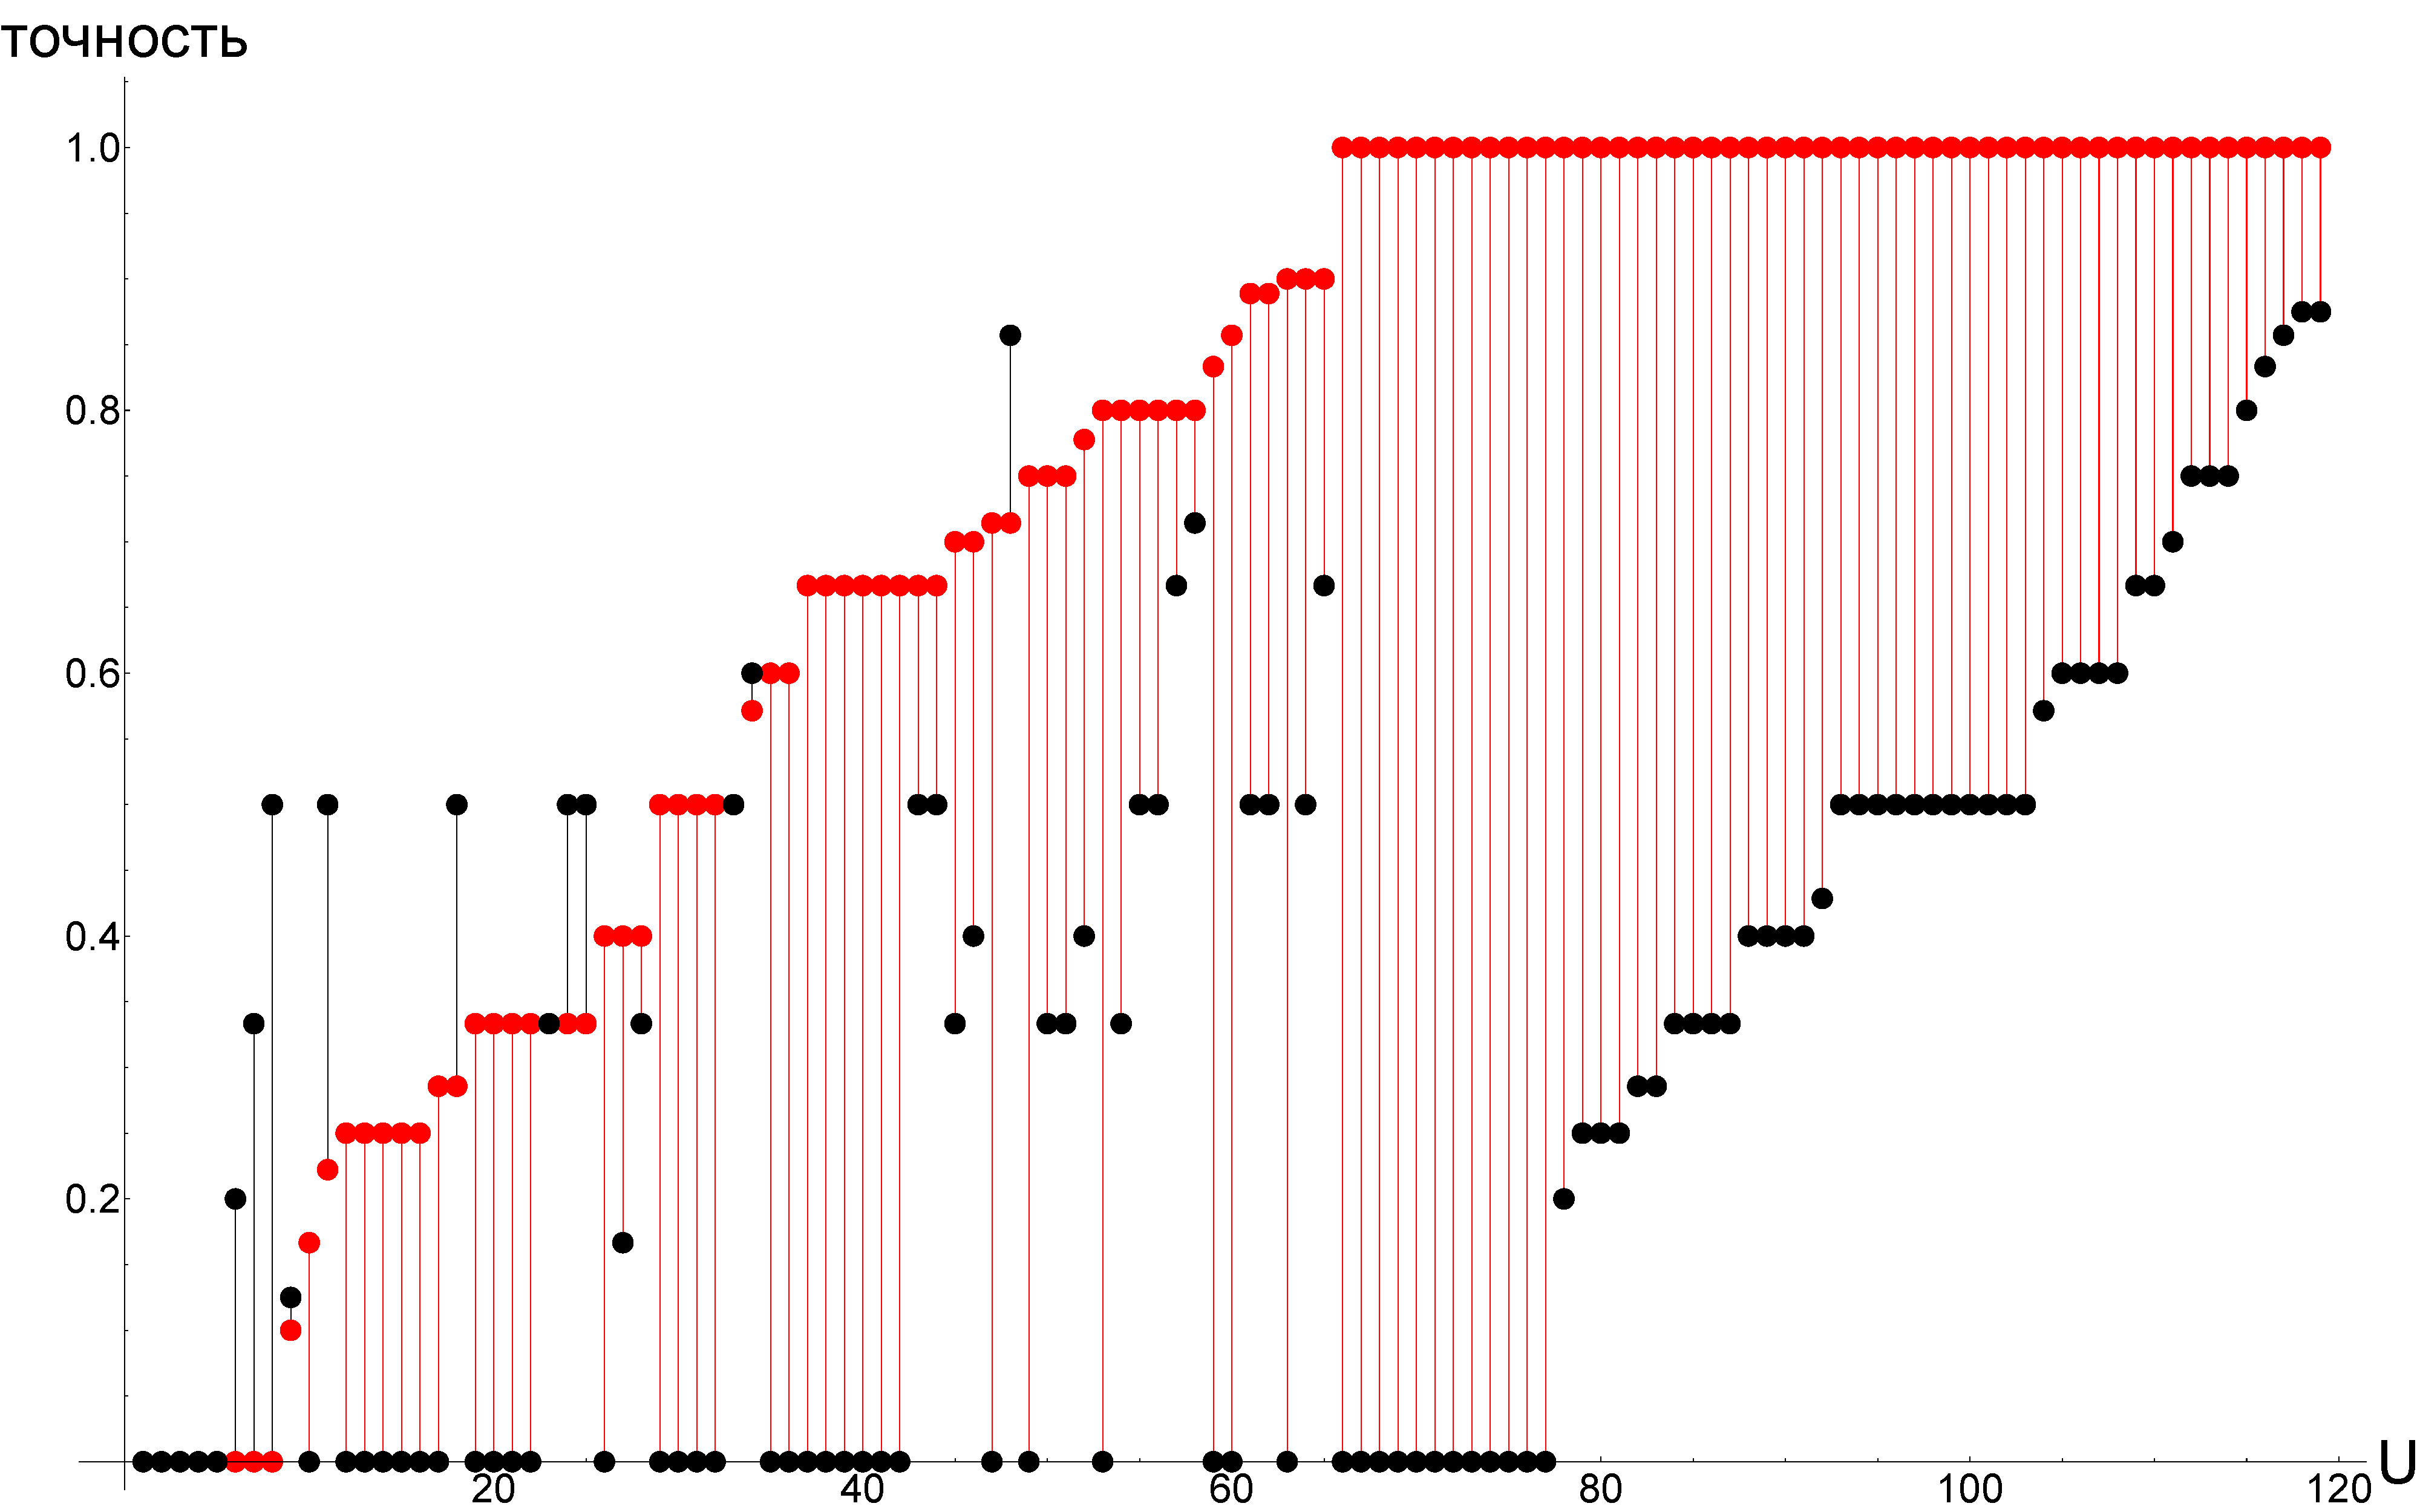
\includegraphics[width=5in,height=2in]{pics/results/ib_method_in_ib_and_fuzzy_model.pdf}
\end{center}
\end{figure}

{\bf Качество решений задачи $topN$ при использовании $\Pi_O$ в ООМ и $\Pi_f$ в
НРС}\\
На Рис. \ref{pic:topn_pio_pif} приведены результаты решения
задачи $topN$ при применении $\Pi_O$ в ООМ и $\Pi_f$ в НРС.
Черным цветом обозначены результаты решения в НРС.
Видно, что НРС более эффективна по критерию качества.

\begin{figure}[H]
	\caption{Качество решений задачи $topN$ при использовании $\Pi_O$ в ООМ и
	$\Pi_f$ в НРС}
	\label{pic:topn_pio_pif}
	\begin{center}
		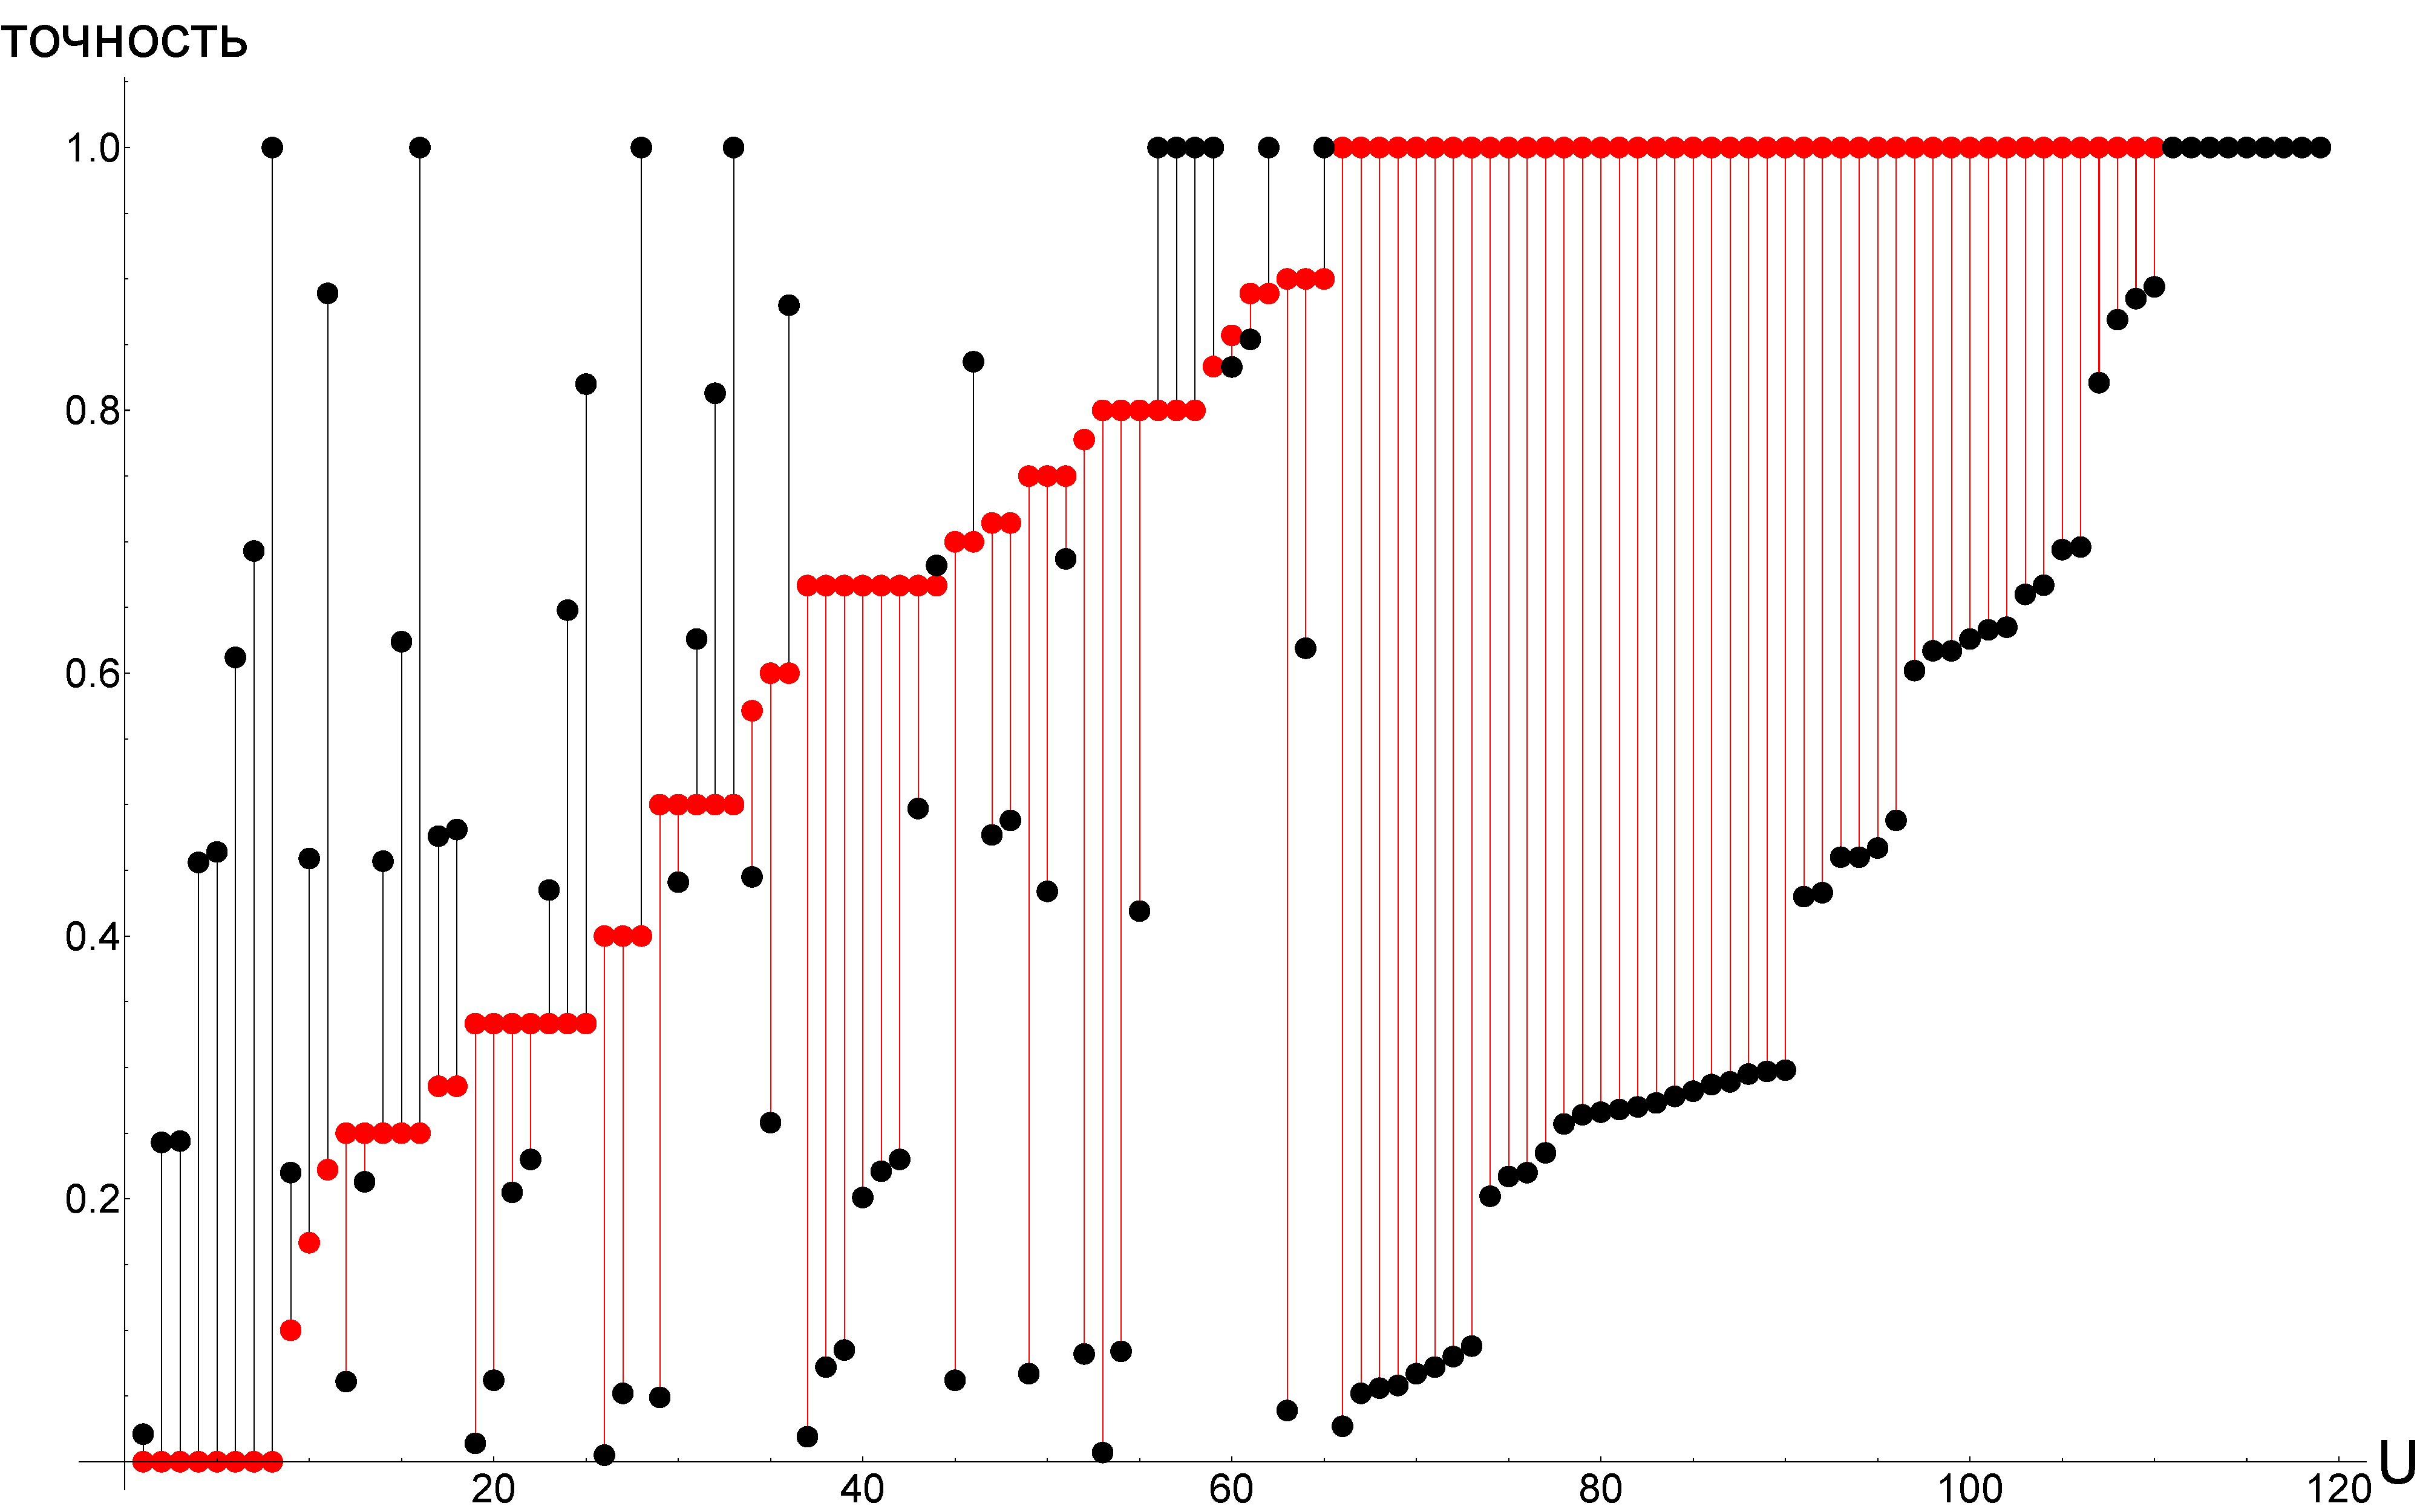
\includegraphics[width=5in,height=2in]{pics/results/topn_oom_fuzz.pdf}
\end{center}
\end{figure}
Видно, что в большинстве НРС более эффективна по критерию качества,
в других ситуациях предпочтения пользователя неоднородны,
и эвристическое предположение, на котором основано построение
функции $\delta_c$, не верно для пользователя.


{\bf Качество решений задачи $pred$ к при использовании $\Pi_C$ в СОМ и НРС}
На Рис. \ref{pic:pred_pic} приведены результаты решения
задачи $pred$ при применении $\Pi_C$ в СОМ и НРС.
Черным цветом обозначены результаты решения в НРС.

\begin{figure}[H]
	\caption{Качество решений задачи $pred$ при использовании $\Pi_C$ в СОМ и
	НРС}
	\label{pic:pred_pic}
	\begin{center}
		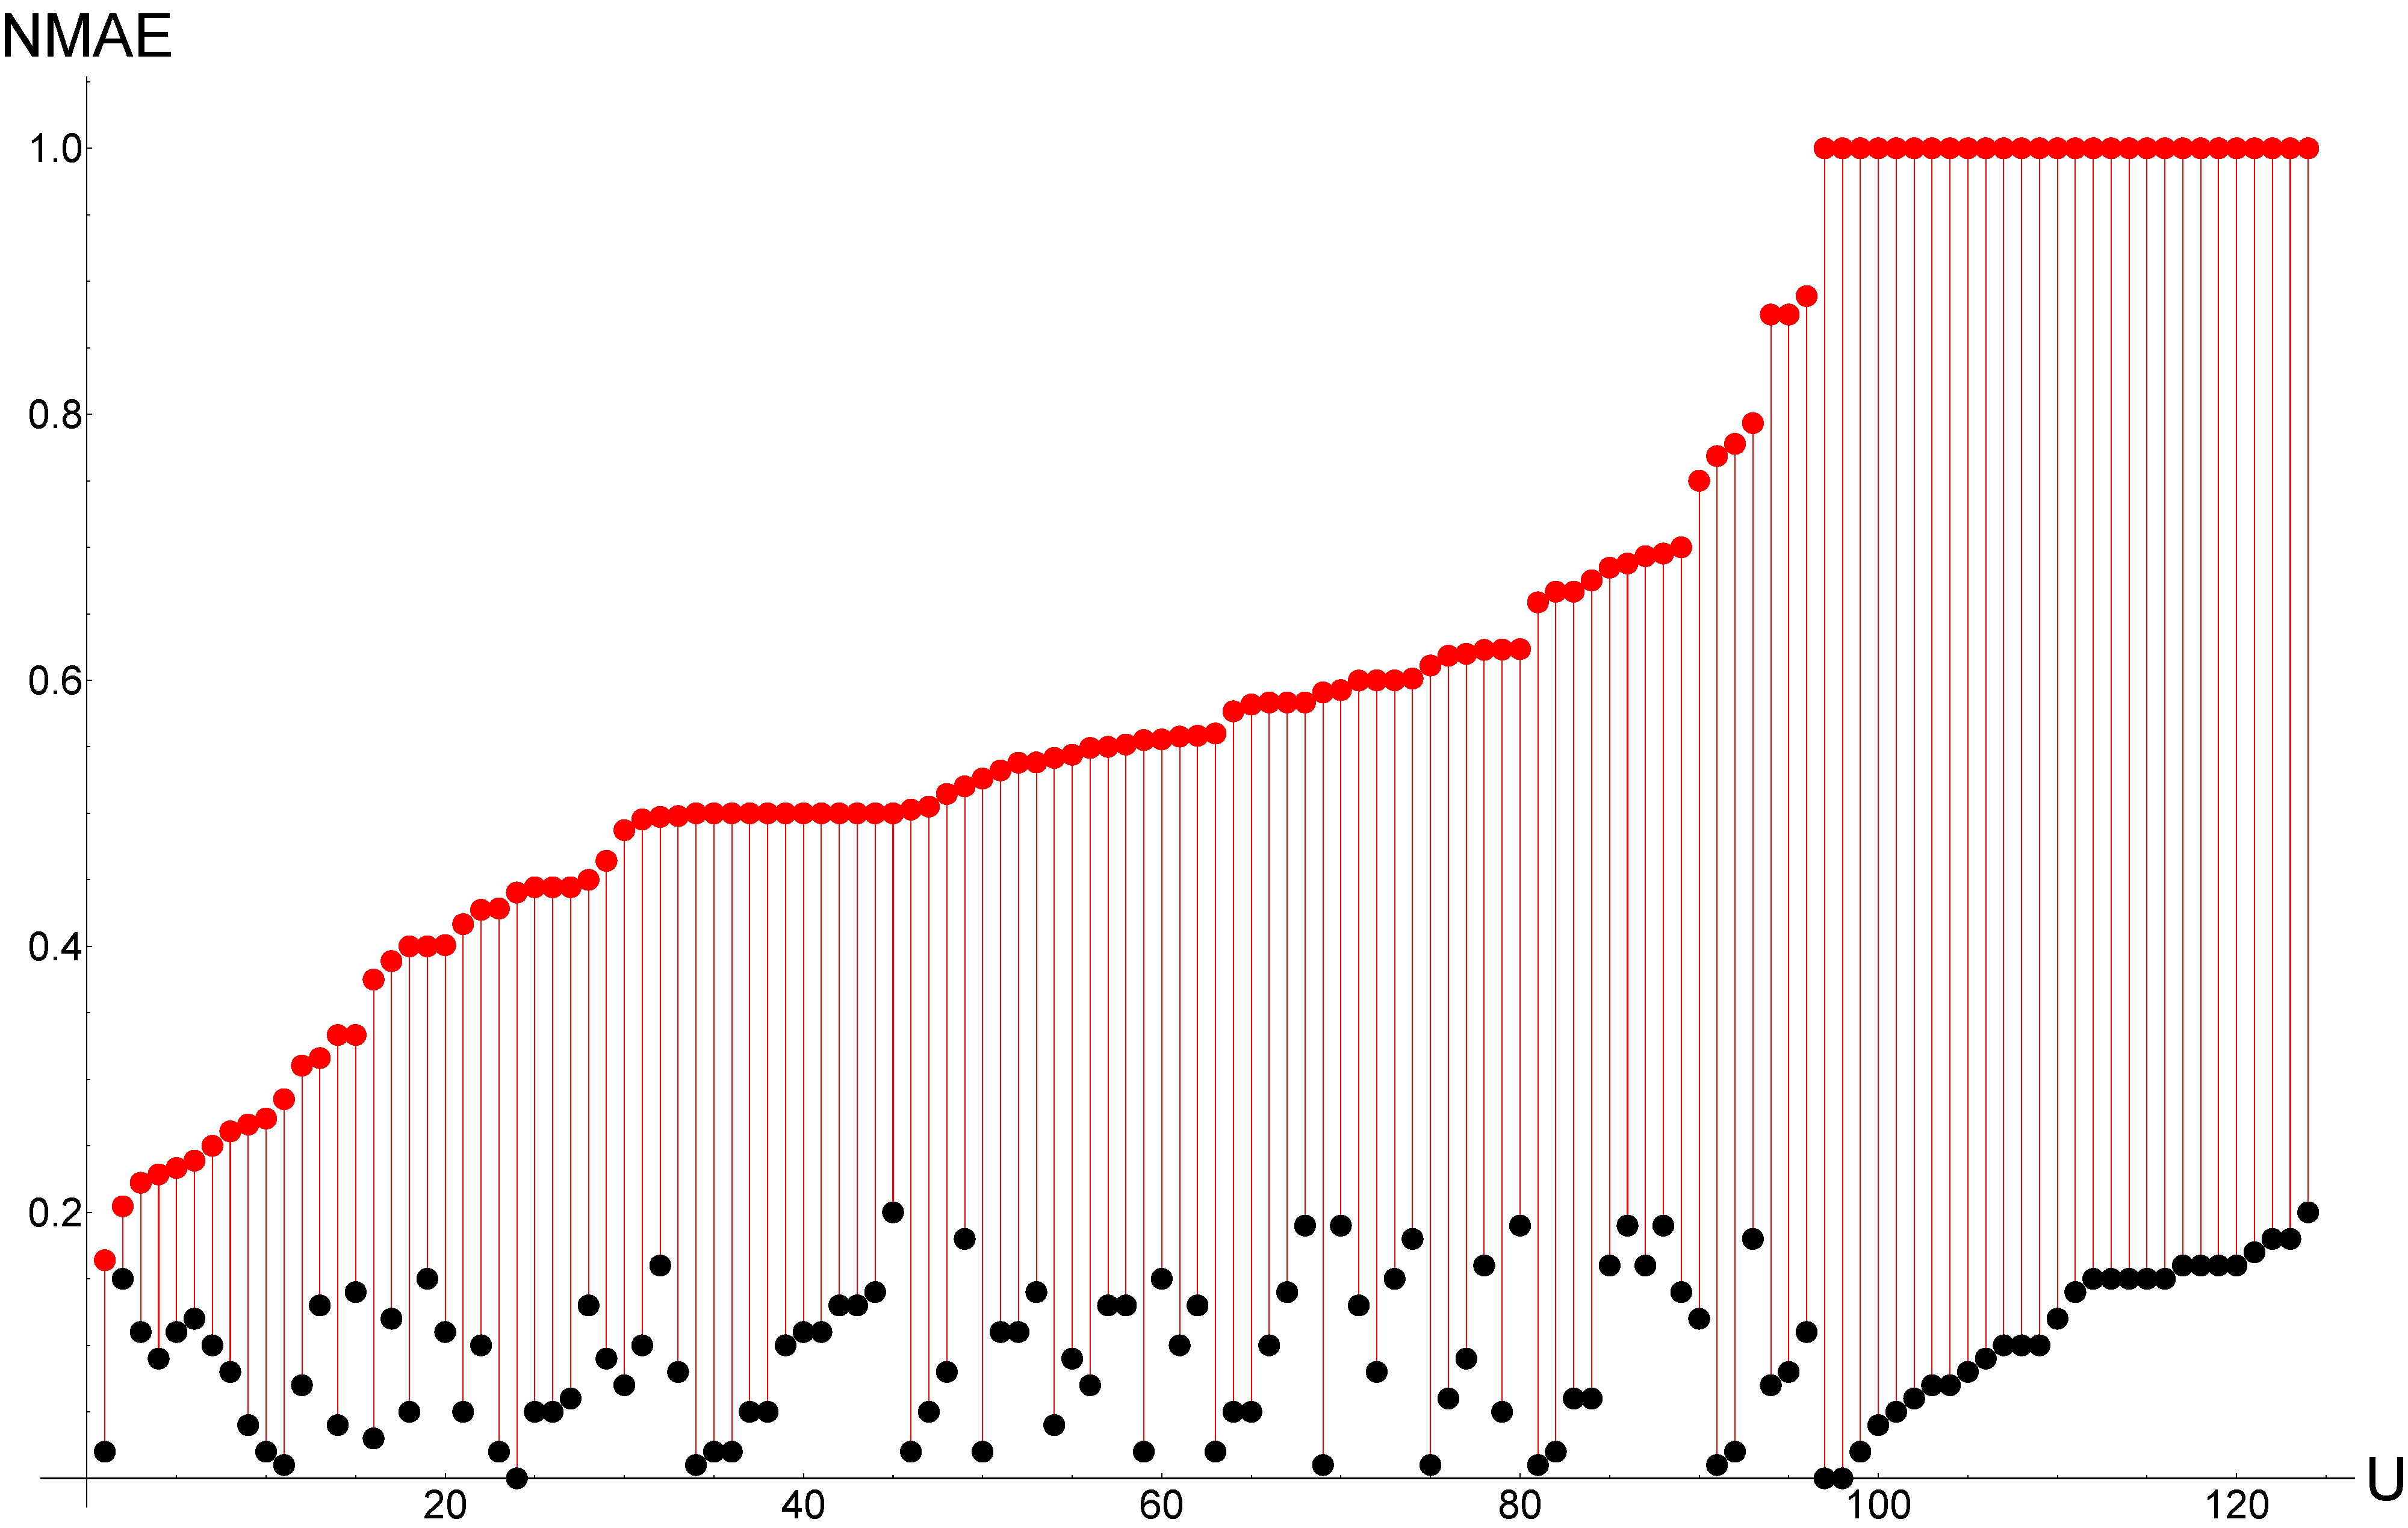
\includegraphics[width=5in,height=2in]{pics/results/ub_method_in_ub_and_fuzz_model.pdf}
\end{center}
\end{figure}
Видно, что в большинстве НРС более эффективна по критерию качества,
в других ситуациях предпочтения пользователя неоднородны.

{\bf Качество решений задачи $pred$ при использовании $\Pi_C$ и $\Pi_f$}
На Рис. \ref{pic:pred_pio_pif} приведены результаты решения
задачи $pred$ при применении $\Pi_C$ в СОМ и $\Pi_f$ в НРС.
Черным цветом обозначены результаты решения в НРС.

\begin{figure}[H]
	\caption{Качество решений задачи $pred$ при использовании $\Pi_C$ в СОМ и
	$\Pi_f$ в НРС}
	\label{pic:pred_pio_pif}
	\begin{center}
		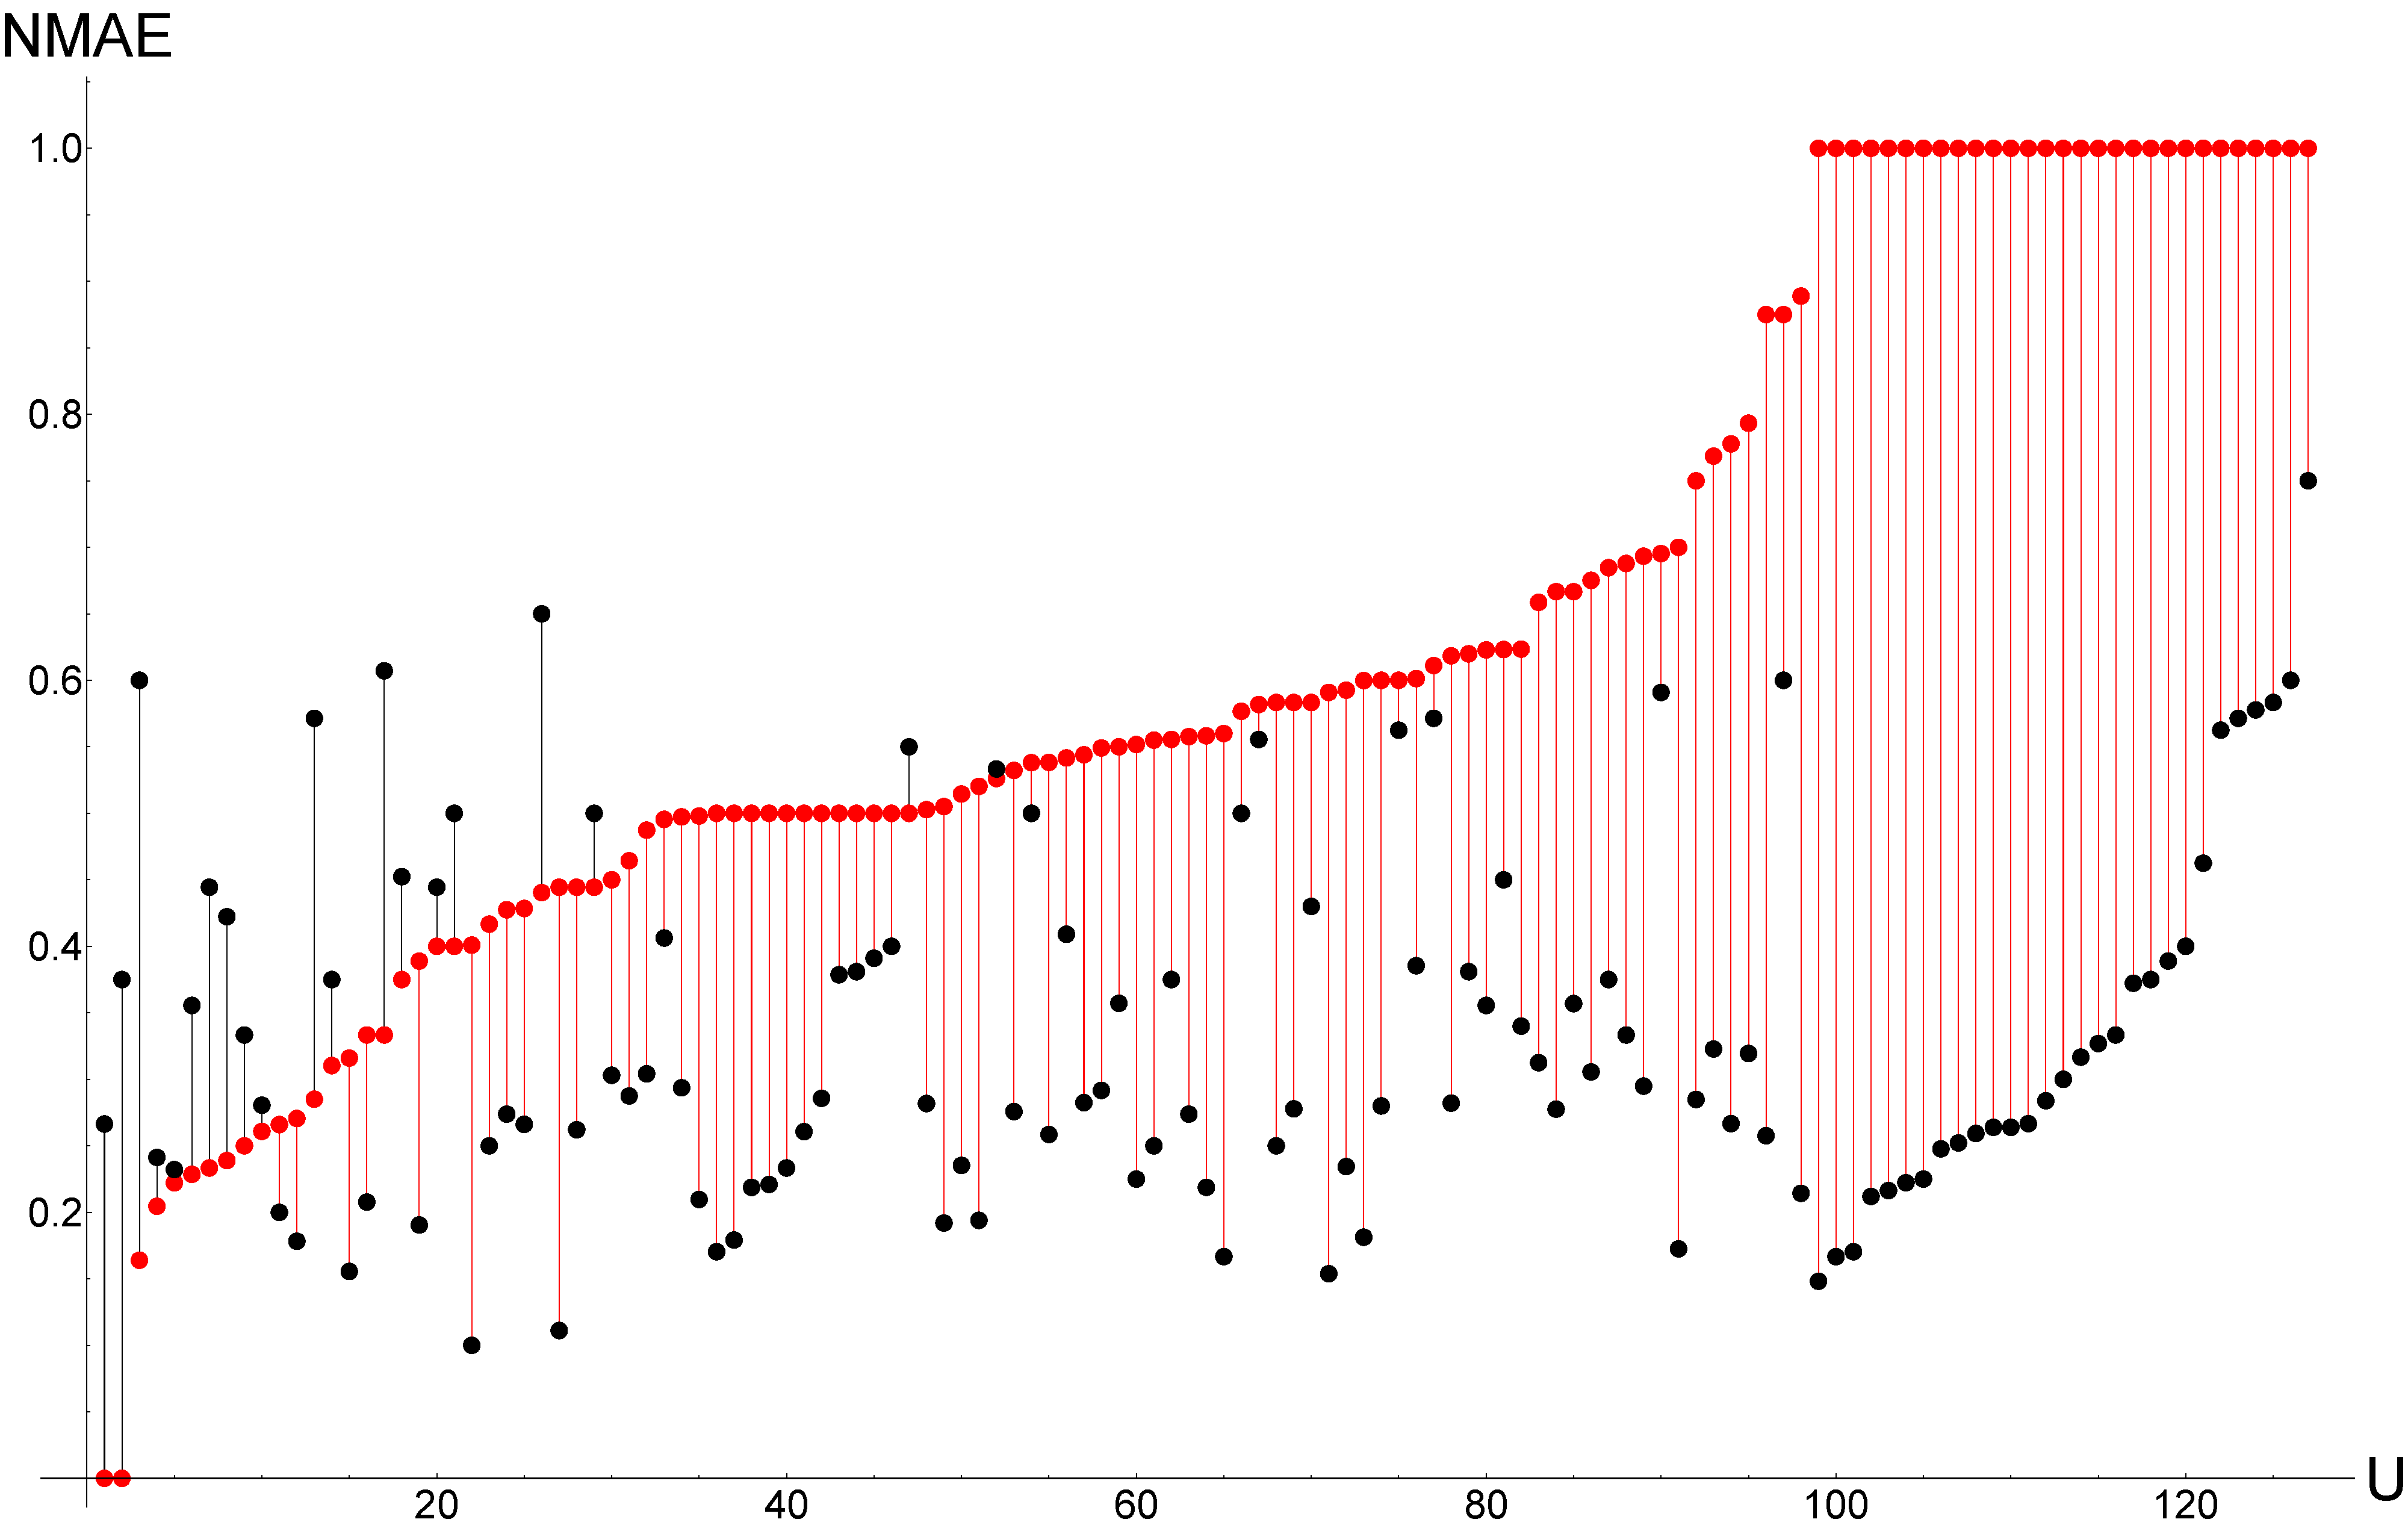
\includegraphics[width=5in,height=2in]{pics/results/ub_vs_fuzzy.pdf}
\end{center}
\end{figure}
Видно, что в большинстве НРС более эффективна по критерию качества,
в других ситуациях предпочтения пользователя неоднородны.
и эвристическое предположение, на котором основано построение
функции $\delta_c$, не верно для пользователя.

%{\bf Влияние свойства неоднородности на качество решения задачи $topN$ в ООМ и
%нечеткой модели}
%На Рис. \ref{pic:topn_trans} приведены результаты решений задачи $topN$ при
%применении $\Pi_O$ в ООМ и $\Pi_f$ и в нечеткой модели. Видно, что 
%
%\begin{figure}[htb]
%	\caption{Влияние свойства транзитивности на ООМ при решении задачи $topN$}
%	\label{pic:topn_trans}
%	\begin{center}
%		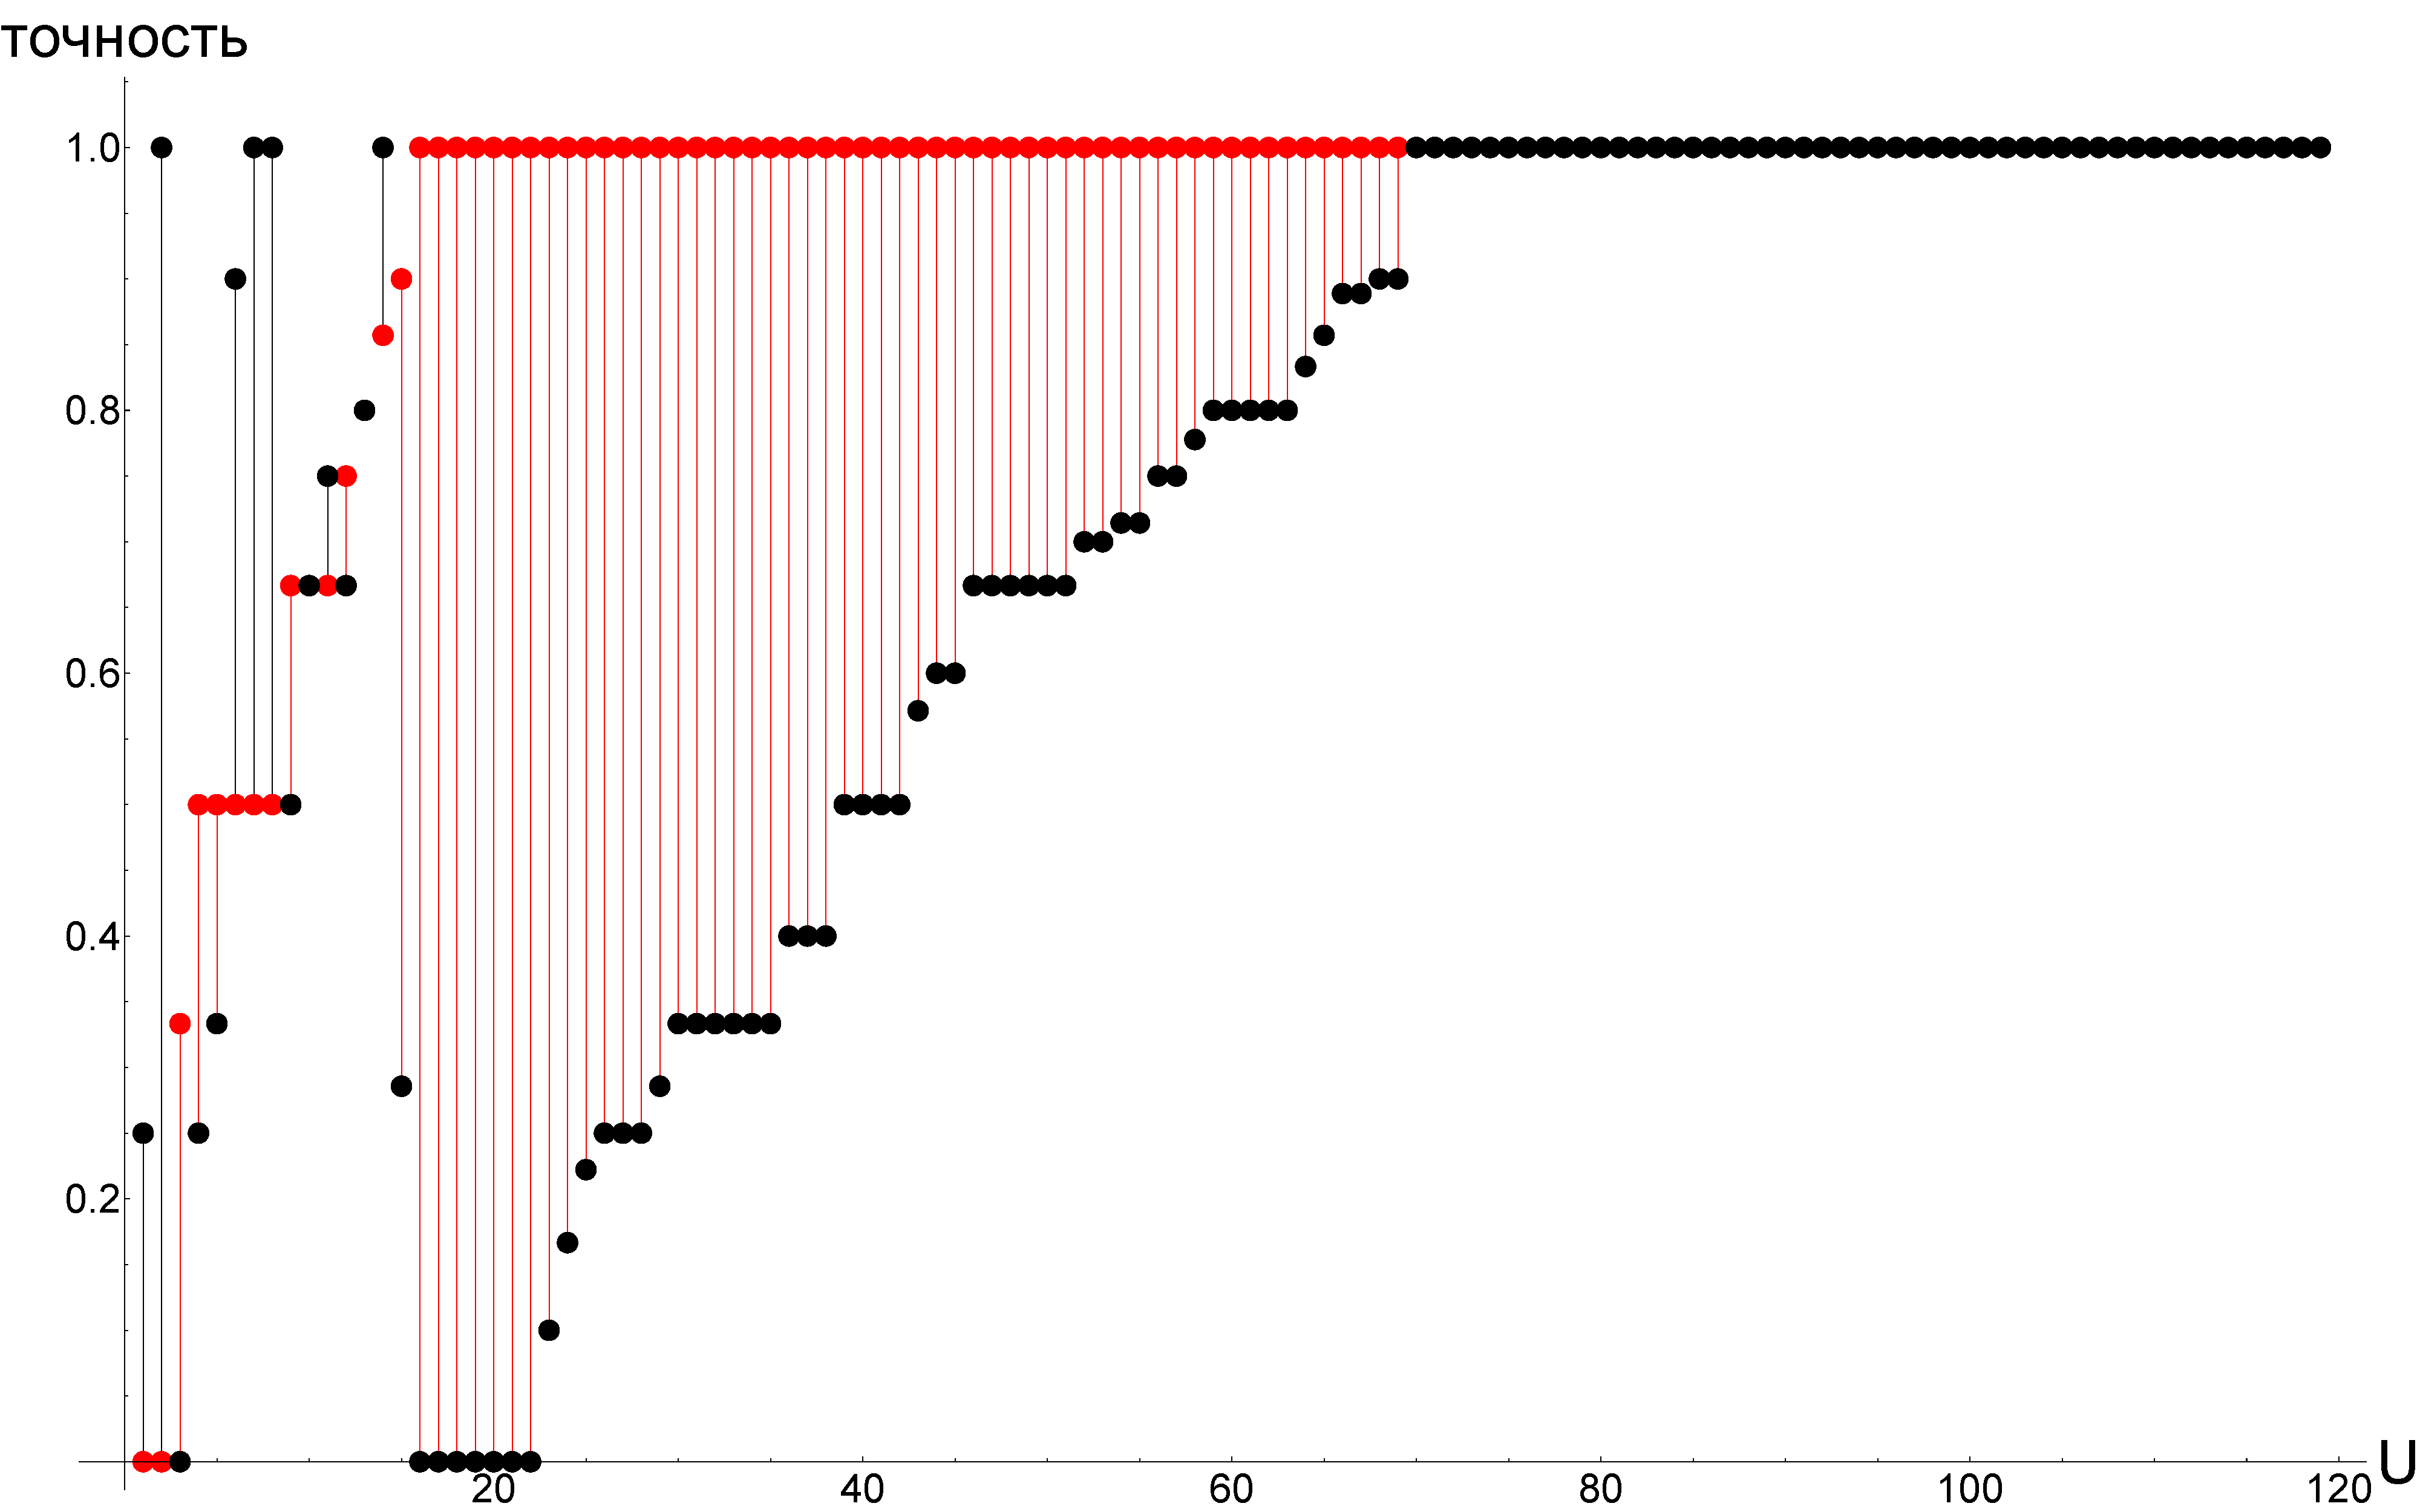
\includegraphics[width=5in,height=2in]{pics/results/transitivity.pdf}
%\end{center}
%\end{figure}



%\subsubsection{Влияние свойства транзитивности}
%В главе, посвященной анализу АКМ было выведено достаточное (\ref{suf-cond-pred-srs}) и
%необходимое (\ref{nec-cond-pred-srs})
%условие, при выполнении которого АКМ гарантируют получение эффективного
%решения. Это условие заключается в том, что на кластере соседей
%должно выполняться свойство транзитивности отношения близости.
%При применении нечеткой модели достаточное и необходимое условия выполняются,
%поэтому результаты решения в ней более эффективны, чем в СОМ.
%
%Выполнение свойства транзитивности зависит от того,
%какая функция используется в качестве меры сходства и какое пороговое
%значение установлено. Проведем следующие тесты:
%
%\begin{enumerate}
%	\item в СОМ при применении стандартного алгоритма решения задачи
%		прогнозирования (\ref{alg:p-srs}), основанного на
%		правиле вывода $\Pi_C$. Пороговое значение $\Delta_u$ равно $0,1$,
%		применяемая мера сходства --- коэффициент корреляции Пирсона
%		(\ref{pearson});
%
%	\item  в СОМ при применении стандартного алгоритма решения задачи
%		прогнозирования (\ref{alg:p-srs}), основанного на
%		правиле вывода $\Pi_C$. Пороговое значение $\Delta_u$ равно $0,5$,
%		применяемая мера сходства --- коэффициент корреляции Пирсона
%\end{enumerate}
%
%Результаты представлены таблицей <<Среднее значение $NMAE$ при различных пороговых значения>> (\ref{tbl:trans-p}), в которой
%указаны средние значения для $NMAE$ по всем пользователям. Среднее значение
%$NMAE$ при использовании $\Delta = 0,1$ на порядок ниже, чем значение
%$NMAE$ при использовании $\Delta = 0,5$.
%Так как при использовании коэффициента корреляции Пирсона,
%если $(\du(u, v) = 1) \wedge (\du(v, z) = 1) \Rightarrow (\du(u, z) =
%1)$, то при пороговом значении $\Delta_u = 0,1 $вероятность того,
%что свойство транзитивности на кластере соседей будет проявляться,
%выше, чем при использовании $\Delta_u = 0,5$.
%
%Практические результаты подтверждают теоретический вывод
%(\ref{suf-cond-pred-srs}, \ref{nec-cond-pred-srs}) о том, что
%от выполнения свойства транзитивности отношения близости зависит
%качество решения задачи прогнозирования в СОМ, а
%выполнение свойства транзитивности зависит от таких параметров,
%как функция, используемая в качестве меры сходства и ее порогового
%значения.
%
%\begin{table}[htb]
%	\caption{Среднее значение $NMAE$ при различных пороговых значения}
%  \begin{center}
%	\label{tbl:trans-p}
%	\begin{tabular}{|c|c|}
%	  \hline
%		Пороговое значение & NMAE \\ \hline
%		0,1&0,495 \\ \hline
%		0,5&0,601 \\ \hline
%	\end{tabular}
%  \end{center}
%\end{table}


%
% =============== OLD ==============
%


%Для решения задач $topN$ и прогнозирования в ООМ и СОМ соответственно
%использовались стандартные алгоритмы и подходы, которые заключаются
%в построении кластера соседей. При решении задачи $topN$ в
%ООМ использовалась мера сходства косинус, при решении задачи прогнозирования
%в СОМ – коэффициент корреляции Пирсона. Те же алгоритмы были применены при
%решении задач в нечеткой модели, но при этом использовались
%расстояния $\rhi$ и $\rhu$ и описанные выше модификации алгоритмов.
%Пороговое значение $\varepsilon_p, \varepsilon_i$ было принято равным 0,1.
%
%Стандартно при проведении тестирования данные о пользователе случайно
%разбивались в следующем отношении: 80\% – обучающее множество,
%20\% – тестовое. Обозначим такое разбиение цифрой 1. Помимо стандартного
%разбиения использовались и другие специально сформированные разбиения 2 и 3.
%Разбиение 2 составлено так, что обучающее множество состоит из таких объектов
%$i$,  для которых выполняется отношение $\rt$, тестовое множество состоит из
%таких объектов $j$, для которых отношение $i \rt j$ не выполняется.
%Такое разбиение создано для того, чтобы подтвердить или опровергнуть
%влияние свойства неоднородности данных на эффективность по критерию качества.
%Разбиение 3 составлено так же, как и стандартное разбиение, но в нем участвуют
%только те пользователи, для которых функция $\delta_c$ задана аккуратно.
%
%Эффективность решений задач по критерию качества определяется усредненными
%по числу тестов (равному 1000 для каждой задачи, разбиению и модели) значениями
%функций, использующихся в РС в качестве оценок.
%Эффективность решения задачи $topN$ по критерию качества оценивалась
%значениями функций точность (P), точность по списку длины L, средняя точность,
%NDCG.
%В результате тестирования среднее значение этих функций мало отличалось,
%поэтому в Таблице \ref{table:topn} приведены только значения точности.
%Большее значение
%точности свидетельствует о то, что решение более эффективно. Эффективность
%решения задачи прогнозирования по критерию качества оценивалась значениями
%функций MAE, NMAE, RMSE, меньшее значение которых говорит о более эффективном
%решении.
%В результате тестирования среднее значение этих функций мало отличалось,
%поэтому в Таблице \ref{table:p} приведены только значения NMAE.
%
%\begin{table}[htb]
%	\caption{Задача $p$}
%  \begin{center}
%	\label{table:p}
%	\begin{tabular}{|c|c|c|c|}
%	  \hline
%		\textnumero & Модель/Правило вычисления & Разбиение & P \\ \hline
%		1&СОМ/$\Pi_{COM}$&1&0,23 \\ \hline
%		2&СОМ/$\Pi_{COM}$&2&0,21 \\ \hline
%		3&Нечеткая СОМ/$\Pi_{COM}$&1&0,13 \\ \hline
%		4&Нечеткая СОМ/$\Pi_{COM}$&2&0,18 \\ \hline
%		5&Нечеткая СОМ/$\Pi_{f}$&1&0,21 \\ \hline
%		6&Нечеткая СОМ/$\Pi_{f}$&2&0,22 \\ \hline
%		7&Нечеткая СОМ/$\Pi_{f}$&3&0,11 \\ \hline
%		8&СОМ$^{\star}$/$\Pi_{COM}$&2&0,15 \\ \hline
%	\end{tabular}
%  \end{center}
%\end{table}
%
%\begin{table}[htb]
%	\caption{Задача $topN$}
%  \begin{center}
%	\label{table:topn}
%	\begin{tabular}{|c|c|c|c|}
%	  \hline
%		\textnumero & Модель/Правило вычисления & Разбиение & NMAE \\ \hline
%		1&ООМ/$\Pi_{OOM}$&1&0,32 \\ \hline
%		2&ООМ/$\Pi_{OOM}$&2&0,24 \\ \hline
%		3&Нечеткая ООМ/$\Pi_{OOM}$&1&0,55 \\ \hline
%		4&Нечеткая ООМ/$\Pi_{OOM}$&2&0,53 \\ \hline
%		5&Нечеткая ООМ/$\Pi_{f}$&1&0,39 \\ \hline
%		6&Нечеткая ООМ/$\Pi_{f}$&2&0,36 \\ \hline
%		7&Нечеткая ООМ/$\Pi_{f}$&3&0,81 \\ \hline
%	\end{tabular}
%  \end{center}
%\end{table}
%
%Прокомментируем данные Таблиц \ref{table:topn} и \ref{table:p}. Результаты 1 эффективней результатов 2 и
%результаты 3 эффективней результатов 4, что подтверждает теоретические выводы
%о влиянии свойства неоднородности на эффективность по критерию качества при
%применении ООМ. Разбиение 2 задано так, что свойства неоднородности влияют на
%эффективность решения, так как между объектами обучающего и тестового
%множеств не выполняется отношение сходства, в результате чего нарушается
%утверждение ООМ (\ref{ors-assert}). Разбиение 2 увеличивает вероятность того, что утверждение
%СОМ (\ref{srs-assert}) может быть неверным, поэтому результаты 1 и 3
%эффективней результатов 2 и 4 Таблицы 2.
%Результаты 3 и 4 эффективней результатов 1 и 2, что подтверждает вывод о том,
%что нечеткая контентная модель является эффективным расширением, так как в
%ней выполняются
%достаточные условия
%1 и 2. Эти же результаты подтверждают выводы о влиянии меры сходства на
%эффективность ООМ и СОМ по критерию качества.
%Результаты 7 эффективней результатов 3–6, так как для разбиения 7 функция
%$\delta_c$
%задана аккуратно. Результаты 7 эффективней результатов 5 и 6, так как для 5 и 6
%в общем случае $\delta_c$  не задана аккуратно, и поэтому же 5 и 6 не
%эффективней 3 и 4. Результаты 5 эффективней 6, так как функция $\delta_c$
%задавалась на основании данных обучающего множества, и поэтому свойство
%неоднородности влияет на аккуратность функции так же, как и на эффективность
%КМ по критерию качества. Использование
%$\Pi_f$ может быть неэффективным, если о пользователях известна только та
%информация, которая
%принадлежит исходному множество P. В такой ситуации эффективней использовать
%нечеткую модель
%$\Pi_{OOM}$ или $\Pi_{COM}$. Для задания функции $\delta_c$ можно использовать
%информацию, которая никак не зависит
%от мощности и свойств исходных данных, и тогда решения задач в нечеткой
%контентной модели не будут
%зависеть от свойств исходных данных. Такой информацией может выступать, к примеру, контекстная информация
%
%Результаты 8 эффективней результатов 1 --- в этом тесте использовался
%модифицированный алгоритм построения кластера соседей\ref{method}.
%Данный результат является следствием того, что на построенном кластере
%выполняется достаточное условие получения эффективного решения по критерию
%качества.
%
